\newpage

\section{Analysis}

\subsection{Users}

The \code{users.csv} file contains records of 19,925,838 (around 20 million) users.

\subsubsection{Exponential Growth}

After launching in 2007, GitHub has seen exponential growth, which is made evident from Figure 1.

\begin{figure}[htb]
\centering
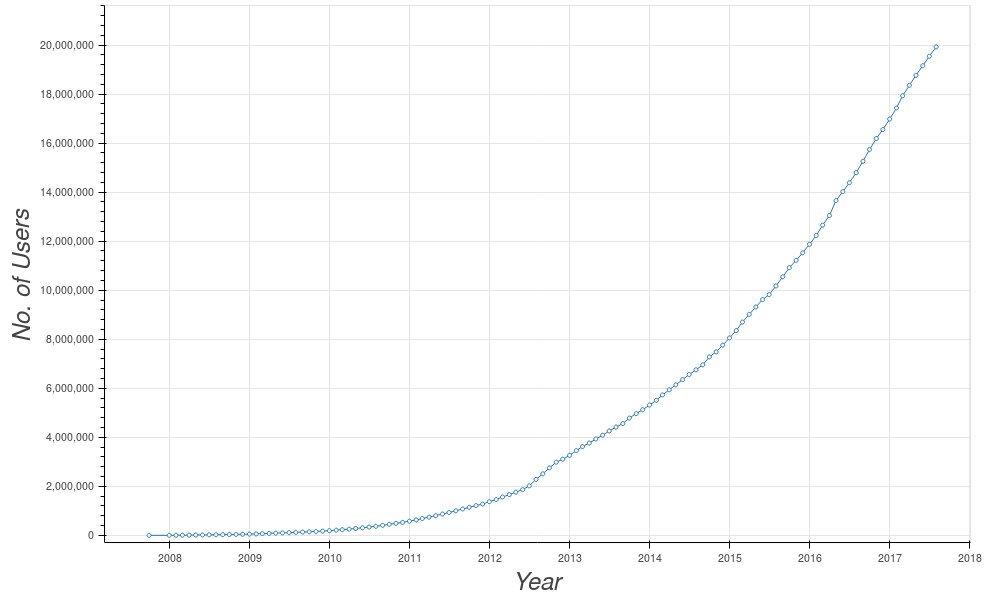
\includegraphics[scale=0.35]{users-exponential-growth}
\caption{User growth rate}
\end{figure}


% \newpage
\subsubsection{New users per Year-Month}

Figure 2 shows that May, 2016 was the month in which most new users were added to the site.

\begin{figure}[htb]
\centering
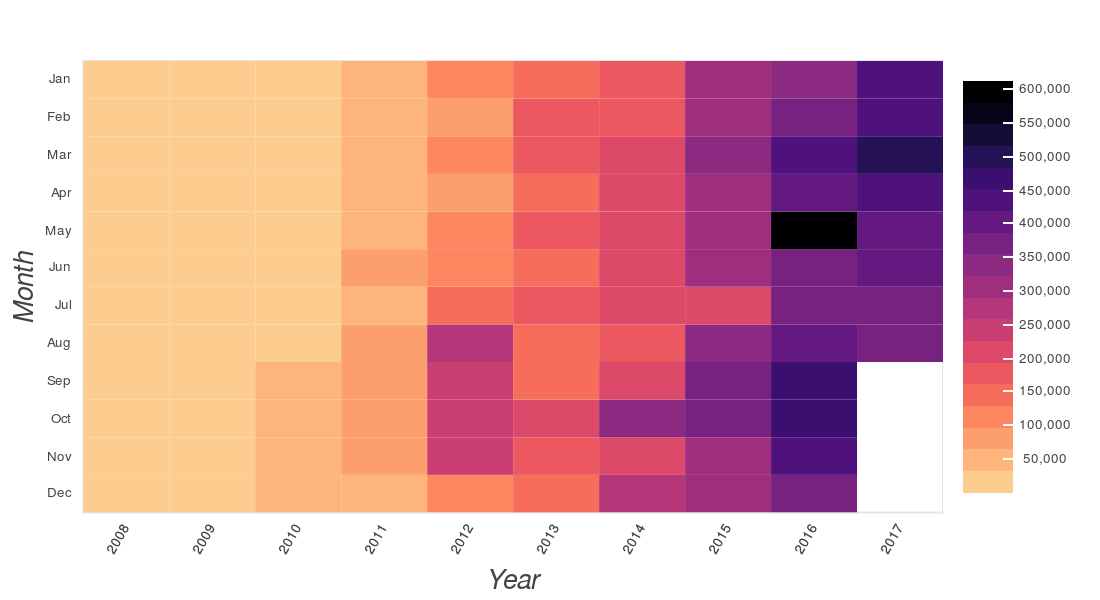
\includegraphics[scale=0.35]{user-year-month}
\caption{New users added per Year-Month}
\end{figure}

\subsubsection{User distribution across countries}

GitHub allows users to enter their location field in a free form text field. Since this user entered data is not validated by GitHub, it can contain anything and does not have to be a valid location. GHTorrent service uses mapping APIs like Bing \& Open Street Maps to convert the text data into known locations. \\

Since not everyone enters their location and or they don't enter it in a valid format, only 7.8\% (1,566,019) users have location data that can be used. \\

Figure 3 tells us that majority of such users are from USA, followed closely by India and China.

% TODO: Pie Chart for countries

\begin{figure}[htb]
\centering
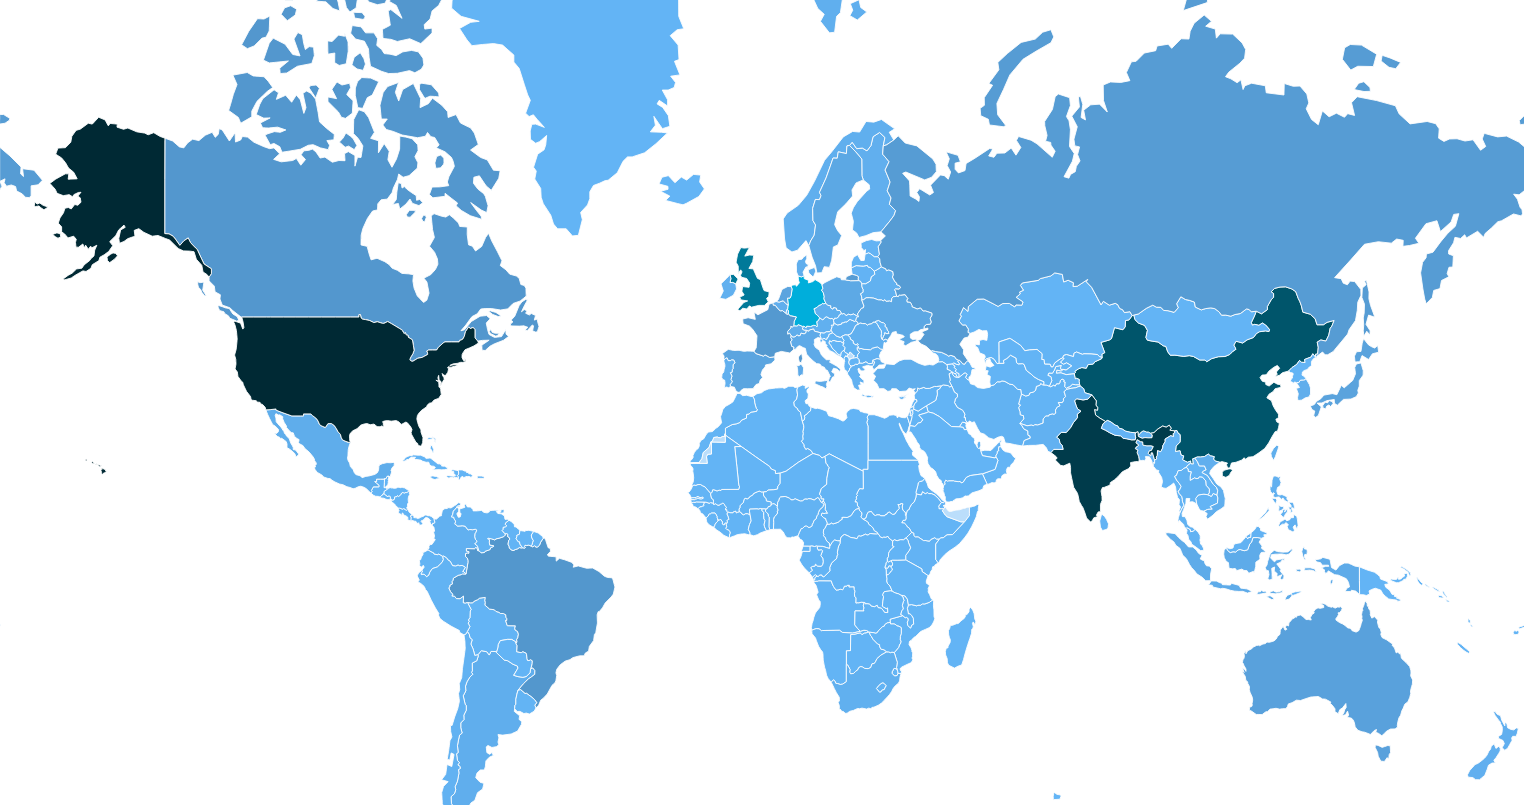
\includegraphics[scale=0.23]{users-country}
\caption{User distribution across countries}
\end{figure}

\subsubsection{User distribution across India}

Of the 1.5 million users with mappable location data, only 102,505 are from India. Their state-wise distribution is given in Figure 4. \\

As can be seen, most github users are from Karnataka and Maharashtra as they are home to IT Hubs like Hyderabad, Bengalore, Pune etc.

\begin{figure}[htb]
\centering
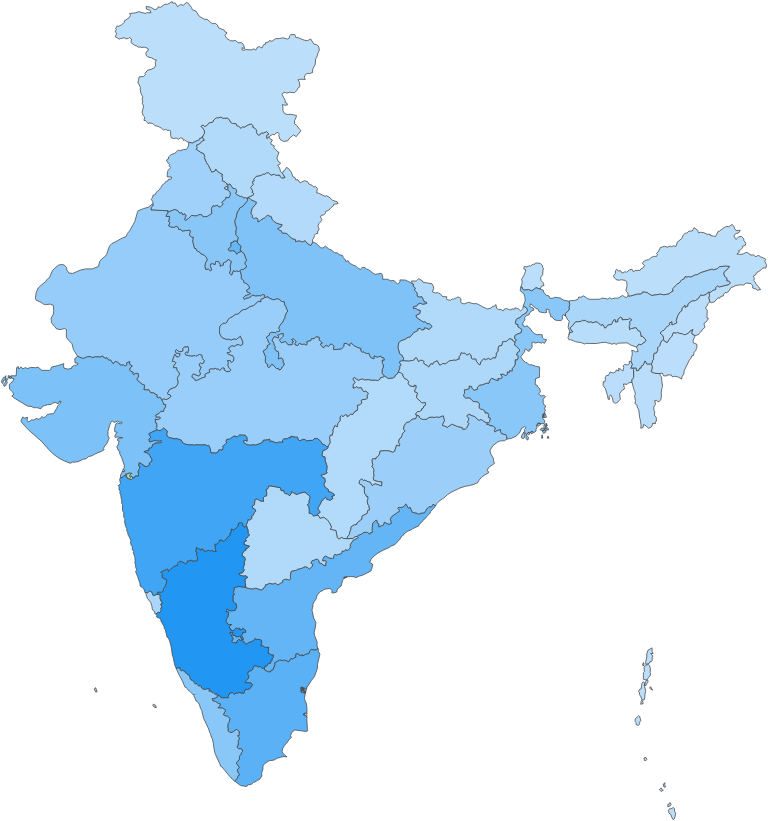
\includegraphics[scale=0.20]{users-india-state}
\caption{User distribution across India}
\end{figure}
